%%%%%%%%%%%%%%%%%%%%% chapter.tex %%%%%%%%%%%%%%%%%%%%%%%%%%%%%%%%%
%
% sample chapter
%
% Use this file as a template for your own input.
%
%%%%%%%%%%%%%%%%%%%%%%%% Springer-Verlag %%%%%%%%%%%%%%%%%%%%%%%%%%
%\motto{Use the template \emph{chapter.tex} to style the various elements of your chapter content.}

\chapter{Rosetta Code Tasks starting with R}

\section*{RSA code}

Given an \href{http://en.wikipedia.org/wiki/RSA}{RSA} key (n,e,d),
construct a program to encrypt and decrypt plaintext messages strings.

\textbf{Background}

RSA code is used to encode secret messages. It is named after Ron
Rivest, Adi Shamir, and Leonard Adleman who published it at MIT in 1977.
The advantage of this type of encryption is that you can distribute the
number ``\emph{n}'' and ``\emph{e}'' (which makes up the Public Key used
for encryption) to everyone. The Private Key used for decryption
``\emph{d}'' is kept secret, so that only the recipient can read the
encrypted plaintext.

The process by which this is done is that a message, for example ``Hello
World'' is encoded as numbers (This could be encoding as ASCII or as a
subset of characters \emph{a} = 01,\emph{b} = 02,\ldots{},\emph{z} =
26). This yields a string of numbers, generally referred to as
``numerical plaintext'', ``\emph{P}''. For example, ``Hello World''
encoded with a=1,\ldots{},z=26 by hundreds would yield
08051212152315181204.

The plaintext must also be split into blocks so that the numerical
plaintext is smaller than \emph{n} otherwise the decryption will fail.

The ciphertext, \emph{C}, is then computed by taking each block of
\emph{P}, and computing

\begin{figure}[H]
\centering

\includegraphics[scale=.6]{graphics/eb1b9606546b68de1ad6063ac988df6c.png}
% \caption{C \textbackslash{}equiv P\^{}e \textbackslash{}mod n}
\end{figure}

Similarly, to decode, one computes

\begin{figure}[H]
\centering
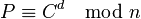
\includegraphics[scale=.6]{graphics/e3a80911ae043c10931e49a6860405d6.png}
% \caption{P \textbackslash{}equiv C\^{}d \textbackslash{}mod n}
\end{figure}

To generate a key, one finds 2 (ideally large) primes \emph{p} and
\emph{q}. the value ``\emph{n}'' is simply:
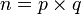
\includegraphics[scale=.6]{graphics/ac0831ae3a81b290afe4473899785ca7.png}.
One must then choose an ``\emph{e}'' such that \\
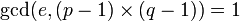
\includegraphics[scale=.6]{graphics/47a50a61203b792b08a69b17c347b73f.png}. \\
That is to say, \emph{e} and
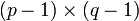
\includegraphics[scale=.6]{graphics/0725da7bdcacd1fcb101173ffeebacae.png}
are relatively prime to each other.

The decryption value \emph{d} is then found by solving

\begin{figure}[H]
\centering
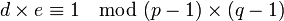
\includegraphics[scale=.6]{graphics/a5e8e37e86ed379e1679034e0235bcd6.png}
% \caption{d\textbackslash{}times e \textbackslash{}equiv 1
% \textbackslash{}mod (p-1)\textbackslash{}times(q-1)}
\end{figure}

The security of the code is based on the secrecy of the Private Key
(decryption exponent) ``\emph{d}'' and the difficulty in factoring
``\emph{n}''. Research into RSA facilitated advances in factoring and a
number of \href{http://www.rsa.com/rsalabs/node.asp?id=2092}{factoring
challenges}. Keys of 768 bits have been successfully factored. While
factoring of keys of 1024 bits has not been demonstrated, NIST expected
them to be factorable by 2010 and now recommends 2048 bit keys going
forward (see
\href{http://en.wikipedia.org/wiki/Key\_size\#Asymmetric\_algorithm\_key\_lengths}{Asymmetric
algorithm key lengths} or
\href{http://csrc.nist.gov/publications/nistpubs/800-57/sp800-57-Part1-revised2\_Mar08-2007.pdf}{NIST
800-57 Pt 1 Revised Table 4: Recommended algorithms and minimum key
sizes}).

\textbf{Summary of the task requirements:}

\begin{itemize}
\item
  Encrypt and Decrypt a short message or two using RSA with a
  demonstration key.
\item
  Implement RSA do not call a library.
\item
  Encode and decode the message using any reversible method of your
  choice (ASCII or a=1,..,z=26 are equally fine).
\item
  Either support blocking or give an error if the message would require
  blocking)
\item
  Demonstrate that your solution could support real keys by using a
  non-trivial key that requires large integer support (built-in or
  libraries). There is no need to include library code but it must be
  referenced unless it is built into the language. The following keys
  will be meet this requirement;however, they are NOT long enough to be
  considered secure:

n = 9516311845790656153499716760847001433441357

e = 65537

d = 5617843187844953170308463622230283376298685

\item
  Messages can be hard-coded into the program, there is no need for
  elaborate input coding.
\item
  Demonstrate that your implementation works by showing plaintext,
  intermediate results, encrypted text, and decrypted text.
\end{itemize}

\begin{wideverbatim}

PicoLisp comes with an RSA library. Usage:

(load "@lib/rsa.l")

# Generate 100-digit keys (private . public)
: (setq Keys (rsaKey 100))
-> (14394597526321726957429995133376978449624406217727317004742182671030....

# Encrypt
: (setq CryptText
   (encrypt (car Keys)
      (chop "The quick brown fox jumped over the lazy dog's back") ) )
-> (72521958974980041245760752728037044798830723189142175108602418861716...

# Decrypt
: (pack (decrypt Keys CryptText))
-> "The quick brown fox jumped over the lazy dog's back"

\end{wideverbatim}

\pagebreak{}
\section*{Random number generator (device)}

If your system has a means to generate random numbers involving not only
a software algorithm (like the \href{http://en.wikipedia.org/wiki//dev/random}{/dev/urandom} devices in
Unix), show how to obtain a random 32-bit number from that mechanism.

\begin{wideverbatim}

: (in "/dev/urandom" (rd 4))
-> 2917110327

\end{wideverbatim}

\pagebreak{}
\section*{Random number generator (included)}

The task is to:

State the type of random number generator algorithm used in a languages
built-in random number generator, or omit the language if no random
number generator is given as part of the language or its immediate
libraries.

If possible, a link to a wider
\href{http://en.wikipedia.org/wiki/List\_of\_random\_number\_generators}{explanation}
of the algorithm used should be given.

Note: the task is \emph{not} to create an RNG, but to report on the
languages in-built RNG that would be the most likely RNG used.

The main types of pseudo-random number generator,
(\href{http://en.wikipedia.org/wiki/PRNG}{PRNG}), that are in use are
the \emph{Linear Congruential Generator},
(\href{http://en.wikipedia.org/wiki/Linear\_congruential\_generator}{LCG}),
and the Generalized Feedback Shift Register,
(\href{http://en.wikipedia.org/wiki/Generalised\_feedback\_shift\_register\#Non-binary\_Galois\_LFSR}{GFSR}),
(of which the
\href{http://en.wikipedia.org/wiki/Mersenne\_twister}{Mersenne
  twister} generator is a subclass). The last main type is where the
output of one of the previous ones (typically a Mersenne twister) is
fed through a \emph{cryptographic hash function} to maximize
unpredictability of individual bits.

Note that LCGs nor GFSRs should be used for the most demanding
applications (cryptography) without additional steps.

\begin{wideverbatim}

PicoLisp uses a linear congruential generator in the built-in (rand) function,
with a multiplier suggested in Knuth's "Seminumerical Algorithms". See the
[http://software-lab.de/doc/refR.html#rand documentation].

\end{wideverbatim}

\pagebreak{}
\section*{Random numbers}

The goal of this task is to generate a collection filled with 1000
normally distributed random (or pseudorandom) numbers with a mean of 1.0
and a \href{http://en.wikipedia.org/wiki/Standard\_deviation}{standard
deviation} of 0.5

Many libraries only generate uniformly distributed random numbers. If
so, use
\href{http://en.wikipedia.org/wiki/Normal\_distribution\#Generating\_values\_from\_normal\_distribution}{this
formula} to convert them to a normal distribution.

\begin{wideverbatim}



(load "@lib/math.l")

(de randomNormal ()  # Normal distribution, centered on 0, std dev 1
   (*/
      (sqrt (* -2.0 (log (rand 0 1.0))))
      (cos (*/ 2.0 pi (rand 0 1.0) `(* 1.0 1.0)))
      1.0 ) )

(seed (time))                                      # Randomize

(let Result
   (make                                           # Build list
      (do 1000                                     # of 1000 elements
         (link (+ 1.0 (/ (randomNormal) 2))) ) )
   (for N (head 7 Result)                          # Print first 7 results
      (prin (format N *Scl) " ") ) )

Output:

1.500334 1.212931 1.095283 0.433122 0.459116 1.302446 0.402477

\end{wideverbatim}

\pagebreak{}
\section*{Range expansion}

A format for expressing an ordered list of integers is to use a comma
separated list of either

\begin{itemize}
\item
  individual integers
\item
  Or a range of integers denoted by the starting integer separated from
  the end integer in the range by a dash, '-'. (The range includes all
  integers in the interval including both endpoints)
\end{itemize}

\begin{itemize}
\item
  \textbf{The range syntax is to be used only for, and for every range
  that expands to more than two values.}
\end{itemize}

\textbf{Example}\\ The list of integers:

-6, -3, -2, -1, 0, 1, 3, 4, 5, 7, 8, 9, 10, 11, 14, 15, 17, 18, 19, 20

Is accurately expressed by the range expression:

-6,-3-1,3-5,7-11,14,15,17-20

(And vice-versa).

The task

Expand the range description:

-6,-3--1,3-5,7-11,14,15,17-20

Note that the second element above, is the \textbf{range from minus 3 to
\emph{minus} 1}.

C.f. \emph{Range extraction}

\begin{wideverbatim}

(de rangeexpand (Str)
   (make
      (for S (split (chop Str) ",")
         (if (index "-" (cdr S))
            (chain
               (range
                  (format (head @ S))
                  (format (tail (- -1 @) S)) ) )
            (link (format S)) ) ) ) )

Output:

: (rangeexpand "-6,-3--1,3-5,7-11,14,15,17-20")
-> (-6 -3 -2 -1 3 4 5 7 8 9 10 11 14 15 17 18 19 20)

\end{wideverbatim}

\pagebreak{}
\section*{Range extraction}

A format for expressing an ordered list of integers is to use a comma
separated list of either

\begin{itemize}
\item
  individual integers
\item
  Or a range of integers denoted by the starting integer separated from
  the end integer in the range by a dash, '-'. (The range includes all
  integers in the interval including both endpoints)
\end{itemize}

\begin{itemize}
\item
  \textbf{The range syntax is to be used only for, and for every range
  that expands to more than two values.}
\end{itemize}

\textbf{Example}\\ The list of integers:

-6, -3, -2, -1, 0, 1, 3, 4, 5, 7, 8, 9, 10, 11, 14, 15, 17, 18, 19, 20

Is accurately expressed by the range expression:

-6,-3-1,3-5,7-11,14,15,17-20

(And vice-versa).

\textbf{The task}

\begin{itemize}
\item
  Create a function that takes a list of integers in increasing order
  and returns a correctly formatted string in the range format.
\item
  Use the function to compute and print the range formatted version of
  the following ordered list of integers:
\end{itemize}

\begin{verbatim}
    0,  1,  2,  4,  6,  7,  8, 11, 12, 14,
   15, 16, 17, 18, 19, 20, 21, 22, 23, 24,
   25, 27, 28, 29, 30, 31, 32, 33, 35, 36,
   37, 38, 39
\end{verbatim}

\begin{itemize}
\item
  Show the output of your program.
\end{itemize}

C.f. \emph{Range expansion}


\begin{wideverbatim}

(de rangeextract (Lst)
   (glue ","
      (make
         (while Lst
            (let (N (pop 'Lst)  M N)
               (while (= (inc M) (car Lst))
                  (setq M (pop 'Lst)) )
               (cond
                  ((= N M) (link N))
                  ((= (inc N) M) (link N M))
                  (T (link (list N '- M))) ) ) ) ) ) )

Output:

: (rangeextract
   (0 1 2 4 6 7 8 11 12 14 15 16 17 18 19 20 21 22
      23 24 25 27 28 29 30 31 32 33 35 36 37 38 39 ) )

-> "0-2,4,6-8,11,12,14-25,27-33,35-39"

\end{wideverbatim}

\pagebreak{}
\section*{Rate counter}

Counting the frequency at which something occurs is a common activity in
measuring performance and managing resources. In this task, we assume
that there is some job which we want to perform repeatedly, and we want
to know how quickly these jobs are being performed.

Of interest is the code that performs the actual measurements. Any other
code (such as job implementation or dispatching) that is required to
demonstrate the rate tracking is helpful, but not the focus.

Multiple approaches are allowed (even preferable), so long as they can
accomplish these goals:

\begin{itemize}
\item
  Run N seconds worth of jobs and/or Y jobs.
\item
  Report at least three distinct times.
\end{itemize}

Be aware of the precision and accuracy limitations of your timing
mechanisms, and document them if you can.

\textbf{See also:} \emph{System time}, \emph{Time a function}

\begin{wideverbatim}

[http://software-lab.de/doc/refU.html#usec usec] returns a relative time in
microseconds. This can be used, for example, to measure the time between two key
strokes

(prin "Hit a key ... ")
(key)
(prinl)
(let Usec (usec)
   (prin "Hit another key ... ")
   (key)
   (prinl)
   (prinl "This took " (format (- (usec) Usec) 6) " seconds") )

Output:

Hit a key ...
Hit another key ...
This took 3.132058 seconds

The [http://software-lab.de/doc/refB.html#bench bench] benchmark function could
also be used. Here we measure the time until a key is pressed

(bench (key))
1.761 sec
-> "a"

\end{wideverbatim}

\pagebreak{}
\section*{Ray-casting algorithm}

Given a point and a polygon, check if the point is inside or outside the
polygon using the
\href{graphics/Point\_in\_polygon\#Ray\_casting\_algorithm}{ray-casting
algorithm}.

A pseudocode can be simply:

\begin{verbatim}
 count ← 0
 foreach side in polygon:
   if ray_intersects_segment(P,side) then
     count ← count + 1
 if is_odd(count) then
   return inside
 else
   return outside
\end{verbatim}

Where the function \texttt{ray\_intersects\_segment} return true if the
horizontal ray starting from the point P intersects the side (segment),
false otherwise.

An intuitive explanation of why it works is that every time we cross a
border, we change ``country'' (inside-outside, or outside-inside), but
the last ``country'' we land on is surely \emph{outside} (since the
inside of the polygon is finite, while the ray continues towards
infinity). So, if we crossed an odd number of borders we was surely
inside, otherwise we was outside; we can follow the ray backward to see
it better: starting from outside, only an odd number of crossing can
give an \emph{inside}: outside-inside, outside-inside-outside-inside,
and so on (the - represents the crossing of a border).

So the main part of the algorithm is how we determine if a ray
intersects a segment. The following text explain one of the possible
ways.

\begin{figure}[H]
  \centering
   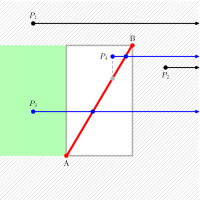
\includegraphics[scale=.6]{graphics/200px-Intersect.png}
\end{figure}

% \emph{\includegraphics[scale=.6]{graphics/magnify-clip.png}}

Looking at the image on the right, we can easily be convinced of the
fact that rays starting from points in the hatched area (like
P\textsubscript{1} and P\textsubscript{2}) surely do not intersect the
segment AB. We also can easily see that rays starting from points in the
greenish area surely intersect the segment AB (like point
P\textsubscript{3}).

So the problematic points are those inside the white area (the box
delimited by the points A and B), like P\textsubscript{4}.

\begin{figure}[H]
  \centering
   
\includegraphics[scale=.6]{graphics/128px-Posslope.png}
\end{figure}


% \emph{\includegraphics[scale=.6]{graphics/magnify-clip.png}}

\begin{figure}[H]
  \centering
   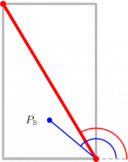
\includegraphics[scale=.6]{graphics/128px-Negslope.png}
\end{figure}

% \emph{\includegraphics[scale=.6]{graphics/magnify-clip.png}}

Let us take into account a segment AB (the point A having y coordinate
always smaller than B's y coordinate, i.e. point A is always below point
B) and a point P. Let us use the cumbersome notation PAX to denote the
angle between segment AP and AX, where X is always a point on the
horizontal line passing by A with x coordinate bigger than the maximum
between the x coordinate of A and the x coordinate of B. As explained
graphically by the figures on the right, if PAX is greater than the
angle BAX, then the ray starting from P intersects the segment AB. (In
the images, the ray starting from P\textsubscript{A} does not intersect
the segment, while the ray starting from P\textsubscript{B} in the
second picture, intersects the segment).

Points on the boundary or ``on'' a vertex are someway special and
through this approach we do not obtain \emph{coherent} results. They
could be treated apart, but it is not necessary to do so.

An algorithm for the previous speech could be (if P is a point, Px is
its x coordinate):

\begin{wideverbatim}
 ray_intersects_segment:
    P : the point from which the ray starts
    A : the end-point of the segment with the smallest y coordinate
        (A must be "below" B)
    B : the end-point of the segment with the greatest y coordinate
        (B must be "above" A)
 if Py = Ay or Py = By then
   Py ← Py + ε
 end if
 if Py < Ay or Py > By then 
   return false
 else if Px > max(Ax, Bx) then 
   return false
 else
   if Px < min(Ax, Bx) then
     return true
   else
     if Ax ≠ Bx then
       m_red ← (By - Ay)/(Bx - Ax)
     else
       m_red ← ∞
     end if
     if Ax ≠ Px then
       m_blue ← (Py - Ay)/(Px - Ax)
     else
       m_blue ← ∞
     end if
     if m_blue ≥ m_red then
       return true
     else
       return false
     end if
   end if
 end if
\end{wideverbatim}

(To avoid the ``ray on vertex'' problem, the point is moved upward of a
small quantity $\varepsilon$)

\begin{wideverbatim}

(scl 4)

(de intersects (Px Py Ax Ay Bx By)
   (when (> Ay By)
      (xchg 'Ax 'Bx)
      (xchg 'Ay 'By) )
   (when (or (= Py Ay) (= Py By))
      (inc 'Py) )
   (and
      (>= Py Ay)
      (>= By Py)
      (>= (max Ax Bx) Px)
      (or
         (> (min Ax Bx) Px)
         (= Ax Px)
         (and
            (<> Ax Bx)
            (>=
               (*/ (- Py Ay) 1.0 (- Px Ax))            # Blue
               (*/ (- By Ay) 1.0 (- Bx Ax)) ) ) ) ) )  # Red

(de inside (Pt Poly)
   (let Res NIL
      (for Edge Poly
         (when (apply intersects Edge (car Pt) (cdr Pt))
            (onOff Res) ) )
      Res ) )

\end{wideverbatim}

\begin{wideverbatim}

Test data:

(de Square
   ( 0.0  0.0  10.0  0.0)
   (10.0  0.0  10.0 10.0)
   (10.0 10.0   0.0 10.0)
   ( 0.0 10.0   0.0  0.0) )

(de SquareHole
   ( 0.0  0.0  10.0  0.0)
   (10.0  0.0  10.0 10.0)
   (10.0 10.0   0.0 10.0)
   ( 0.0 10.0   0.0  0.0)
   ( 2.5  2.5   7.5  2.5)
   ( 7.5  2.5   7.5  7.5)
   ( 7.5  7.5   2.5  7.5)
   ( 2.5  7.5   2.5  2.5) )

(de Strange
   ( 0.0  0.0   2.5  2.5)
   ( 2.5  2.5   0.0 10.0)
   ( 0.0 10.0   2.5  7.5)
   ( 2.5  7.5   7.5  7.5)
   ( 7.5  7.5  10.0 10.0)
   (10.0 10.0  10.0  0.0)
   (10.0  0.0   2.5  2.5) )

(de Exagon
   ( 3.0  0.0   7.0  0.0)
   ( 7.0  0.0  10.0  5.0)
   (10.0  5.0   7.0 10.0)
   ( 7.0 10.0   3.0 10.0)
   ( 3.0 10.0   0.0  5.0)
   ( 0.0  5.0   3.0  0.0) )


Output:

: (inside (5.0 . 5.0) Square)
-> T
: (inside (5.0 . 8.0) Square)
-> T
: (inside (-10.0 . 5.0) Square)
-> NIL
: (inside (0.0 . 5.0) Square)
-> NIL
: (inside (10.0 . 5.0) Square)
-> T
: (inside (8.0 . 5.0) Square)
-> T
: (inside (10.0 . 10.0) Square)
-> NIL

\end{wideverbatim}

\begin{wideverbatim}

: (inside (5.0 . 5.0) SquareHole)
-> NIL
: (inside (5.0 . 8.0) SquareHole)
-> T
: (inside (-10.0 . 5.0) SquareHole)
-> NIL
: (inside (0 . 5.0) SquareHole)
-> NIL
: (inside (10.0 . 5.0) SquareHole)
-> T
: (inside (8.0 . 5.0) SquareHole)
-> T
: (inside (10.0 . 10.0) SquareHole)
-> NIL

: (inside (5.0 . 5.0) Strange)
-> T
: (inside (5.0 . 8.0) Strange)
-> NIL
: (inside (-10.0 . 5.0) Strange)
-> NIL
: (inside (0 . 5.0) Strange)
-> NIL
: (inside (10.0 . 5.0) Strange)
-> T
: (inside (8.0 . 5.0) Strange)
-> T
: (inside (10.0 . 10.0) Strange)
-> NIL

: (inside (5.0 . 5.0) Exagon)
-> T
: (inside (5.0 . 8.0) Exagon)
-> T
: (inside (-10.0 . 5.0) Exagon)
-> NIL
: (inside (0.0 . 5.0) Exagon)
-> NIL
: (inside (10.0 . 5.0) Exagon)
-> T
: (inside (8.0 . 5.0) Exagon)
-> T
: (inside (10.0 . 10.0) Exagon)
-> NIL

\end{wideverbatim}

\pagebreak{}
\section*{Read a configuration file}

The task is to read a configuration file in standard configuration file,
and set variables accordingly. For this task, we have a configuration
file as follows:

\begin{wideverbatim}
# This is a configuration file in standard configuration file format
#
# Lines begininning with a hash or a semicolon are ignored by the application
# program. Blank lines are also ignored by the application program.

# This is the fullname parameter
FULLNAME Foo Barber

# This is a favourite fruit
FAVOURITEFRUIT banana

# This is a boolean that should be set
NEEDSPEELING

# This boolean is commented out
; SEEDSREMOVED

# Configuration option names are not case sensitive, but configuration parameter
# data is case sensitive and may be preserved by the application program.

# An optional equals sign can be used to separate configuration parameter data
# from the option name. This is dropped by the parser. 

# A configuration option may take multiple parameters separated by commas.
# Leading and trailing whitespace around parameter names and parameter data fields
# are ignored by the application program.

OTHERFAMILY Rhu Barber, Harry Barber
\end{wideverbatim}

For the task we need to set four variables according to the
configuration entries as follows:

\begin{itemize}
\item
  fullname = Foo Barber
\item
  favouritefruit = banana
\item
  needspeeling = true
\item
  seedsremoved = false
\end{itemize}

We also have an option that contains multiple parameters. These may be
stored in an array.

\begin{itemize}
\item
  otherfamily(1) = Rhu Barber
\item
  otherfamily(2) = Harry Barber
\end{itemize}


\begin{wideverbatim}

'read' supports only a single comment character. Therefore, we use a pipe to
filter the comments.

(de rdConf (File)
   (pipe (in File (while (echo "#" ";") (till "^J")))
      (while (read)
         (set @ (or (line T) T)) ) ) )

Test:

(off FULLNAME FAVOURITEFRUIT NEEDSPEELING SEEDSREMOVED OTHERFAMILY)
(rdConf "conf.txt")

Output:

: (list FULLNAME FAVOURITEFRUIT NEEDSPEELING SEEDSREMOVED OTHERFAMILY)
-> ("Foo Barber" "banana" T NIL "Rhu Barber, Harry Barber")

\end{wideverbatim}

\pagebreak{}
\section*{Read a specific line from a file}

Some languages have special semantics for obtaining a known line number
from a file. The task is to demonstrate how to obtain the contents of a
specific line within a file. For the purpose of this task demonstrate
how to the contents of the seventh line of a file can be obtained, and
store this in a variable or in memory (for potential future use within
the program if the code were to become embedded). If the file does not
contain seven lines, or the seventh line is empty, or too big to be
retrieved, output an appropriate message. If no special semantics are
available for obtaining the required line, it is permissible to read
line by line. Note that empty lines are considered and should still be
counted. Note that for functional languages or languages without
variables or storage, it is permissible to output the extracted data to
standard output.

\begin{wideverbatim}

(in "file.txt"
   (do 6 (line))
   (or (line) (quit "No 7 lines")) )

\end{wideverbatim}

\pagebreak{}
\section*{Read entire file}

Load the entire contents of some text file as a single string variable.

If applicable, discuss: encoding selection, the possibility of
memory-mapping.

Of course, one should avoid reading an entire file at once if the file
is large and the task can be accomplished incrementally instead (in
which case check \emph{File IO}); this is for those
cases where having the entire file is actually what is wanted.


\begin{wideverbatim}

Using '[http://software-lab.de/doc/refT.html#till till]' is the shortest way:

   (in "file" (till NIL T))

To read the file into a list of characters:

   (in "file" (till NIL))

or, more explicit:

   (in "file" (make (while (char) (link @))))

Encoding is always assumed to be UTF-8.

\end{wideverbatim}

\pagebreak{}
\section*{Read a file line by line}


Read a file one line at a time, as opposed to
\emph{reading the entire file at once}.

See also: \emph{Input loop}.



\begin{wideverbatim}

(in "foobar.txt"
   (while (line)
      (process @) ) )

\end{wideverbatim}

\pagebreak{}
\section*{Real constants and functions}

Show how to use the following math constants and functions in your
language (if not available, note it):

\begin{itemize}
\item
  \emph{e} (Euler's number)
\item
  $\pi$
\item
  square root
\item
  logarithm (any base allowed)
\item
  exponential (\emph{e}\textsuperscript{\emph{x}})
\item
  absolute value (a.k.a. ``magnitude'')
\item
  floor (largest integer less than or equal to this number--not the same
  as truncate or int)
\item
  ceiling (smallest integer not less than this number--not the same as
  round up)
\item
  power (\emph{x}\textsuperscript{\emph{y}})
\end{itemize}

See also \emph{Trigonometric Functions}


\begin{wideverbatim}

PicoLisp has only limited floating point support (scaled bignum arithmetics). It
can handle real numbers with as many positions after the decimal point as
desired, but is practically limited by the precision of the C-library functions
(about 16 digits). The default precision is six, and can be changed with
'[http://software-lab.de/doc/refS.html#scl scl]':

(scl 12)  # 12 places after decimal point
(load "@lib/math.l")

(prinl (format (exp 1.0) *Scl))        # e, exp
(prinl (format pi *Scl))               # pi

(prinl (format (pow 2.0 0.5) *Scl))    # sqare root
(prinl (format (sqrt (* 2.0 1.0)) *Scl))

(prinl (format (log 2.0) *Scl))        # logarithm
(prinl (format (exp 4.0) *Scl))        # exponential

(prinl (format (abs -7.2) *Scl))       # absolute value
(prinl (abs -123))

(prinl (format (pow 3.0 4.0) *Scl))    # power

Output:

2.718281828459
3.141592653590
1.414213562373
1.414213562373
0.693147180560
54.598150033144
7.200000000000
123
81.000000000000

"floor" and "ceiling" are currently not available.

\end{wideverbatim}

\pagebreak{}
\section*{Record sound}

Record a monophonic 16-bit PCM sound into either memory space, a file
or array.

(This task neglects to specify the sample rate, and whether to use
signed samples. The programs in this page might use signed 16-bit or
unsigned 16-bit samples, at 8000 Hz, 44100 Hz, or any other sample
rate. Therefore, these programs might not record sound in the same
format.)


\begin{wideverbatim}

(in '(rec -q -c1 -tu16 - trim 0 2)  # Record 2 seconds
   (make
      (while (rd 2)
         (link @) ) ) )

Output:

-> (16767 19071 17279 ... 5503 9343 14719)  # 96000 numbers

\end{wideverbatim}

\pagebreak{}
\section*{Reduced row echelon form}

Show how to compute the \textbf{reduced row echelon form} (a.k.a.
\textbf{row canonical form}) of a matrix. The matrix can be stored in
any datatype that is convenient (for most languages, this will probably
be a two-dimensional array). Built-in functions or this pseudocode (from
Wikipedia) may be used:

\begin{wideverbatim}
function ToReducedRowEchelonForm(Matrix M) is
    lead := 0
    rowCount := the number of rows in M
    columnCount := the number of columns in M
    for 0 ≤ r < rowCount do
        if columnCount ≤ lead then
            stop
        end if
        i = r
        while M[i, lead] = 0 do
            i = i + 1
            if rowCount = i then
                i = r
                lead = lead + 1
                if columnCount = lead then
                    stop
                end if
            end if
        end while
        Swap rows i and r
        If M[r, lead] is not 0 divide row r by M[r, lead]
        for 0 ≤ i < rowCount do
            if i ≠ r do
                Subtract M[i, lead] multiplied by row r from row i
            end if
        end for
        lead = lead + 1
    end for
end function
\end{wideverbatim}

\pagebreak{}
For testing purposes, the RREF of this matrix:

\begin{verbatim}
 1   2   -1   -4
 2   3   -1  -11
-2   0   -3   22
\end{verbatim}

is:

\begin{verbatim}
1   0   0   -8
0   1   0    1
0   0   1   -2
\end{verbatim}


\begin{wideverbatim}

(de reducedRowEchelonForm (Mat)
   (let (Lead 1  Cols (length (car Mat)))
      (for (X Mat X (cdr X))
         (NIL
            (loop
               (T (seek '((R) (n0 (get R 1 Lead))) X)
                  @ )
               (T (> (inc 'Lead) Cols)) ) )
         (xchg @ X)
         (let D (get X 1 Lead)
            (map
               '((R) (set R (/ (car R) D)))
               (car X) ) )
         (for Y Mat
            (unless (== Y (car X))
               (let N (- (get Y Lead))
                  (map
                     '((Dst Src)
                        (inc Dst (* N (car Src))) )
                     Y
                     (car X) ) ) ) )
         (T (> (inc 'Lead) Cols)) ) )
   Mat )

Output:

(reducedRowEchelonForm
   '(( 1  2  -1   -4) ( 2  3  -1  -11) (-2  0  -3   22)) )
-> ((1 0 0 -8) (0 1 0 1) (0 0 1 -2))

\end{wideverbatim}

\pagebreak{}
\section*{Regular expressions}

The goal of this task is

\begin{itemize}
\item
  to match a string against a regular expression
\item
  to substitute part of a string using a regular expression
\end{itemize}


\begin{wideverbatim}

1. Calling the C library

PicoLisp doesn't have built-in regex functionality.
It is easy to call the native C library.

(let (Pat "a[0-9]z"  String "a7z")
   (use Preg
      (native "@" "regcomp" 'I '(Preg (64 B . 64)) Pat 1)  # Compile regex
      (when (=0 (native "@" "regexec" 'I (cons NIL (64) Preg) String 0 0 0))
         (prinl "String \"" String "\" matches regex \"" Pat "\"") ) ) )

Output:

String "a7z" matches pattern "a[0-9]z"

2. Using Pattern Matching

Regular expressions are static and inflexible. Another possibility is
dynamic pattern matching, where arbitrary conditions can be programmed.

(let String "The number <7> is incremented"
   (use (@A @N @Z)
      (and
         (match '(@A "<" @N ">"  @Z) (chop String))
         (format @N)
         (prinl @A "<" (inc @) ">" @Z) ) ) )

Output:

The number <8> is incremented

\end{wideverbatim}

\pagebreak{}
\section*{Remote agent/Agent interface}

In \emph{Remote agent}, a component is described that marshals
commands and events between a stream and a program that issues
commands and processes the resulting events. Using the protocol
definition described there, build this component in a fashion
idiomatic and natural to your language.

\begin{wideverbatim}

The interface logic for the PicoLisp solution is directly integrated into
the client [[Remote agent/Agent logic#PicoLisp]].

\end{wideverbatim}

\pagebreak{}
\section*{Remote agent/Agent logic}

In \emph{Remote agent}, a game is described where an agent interacts
with a simple world of walls, balls and squares, and a component is
described that marshals commands between the simulation environment
and the logic code behind the agent.

The goal conditions for the game are to get all balls in squares of
matching colors, in as few turns as possible.

Using an \emph{interface} for your language write a program that
attempts to reach these goals. The exact agent behavior within the
simulated environment is unspecified.


\begin{wideverbatim}

This is the client. For the server, see [[Remote agent/Simulation#PicoLisp]].

# Global variables:
#  '*Sock' is the TCP socket to the server
#  '*Dir' is a circular list of direction structures
#  '*World' holds the explored world
#  '*Ball' is the ball found in current field
#  '*Todo' is the list of mismatching fields and balls

(load "@lib/simul.l")

(de *Dir .
   ((north south . extendNorth) (east west . extendEast)
      (south north . extendSouth) (west east . extendWest) . ) )

\end{wideverbatim}

\begin{wideverbatim}

(de gameClient (Host Port)
   (unless (setq *Sock (connect Host Port))
      (quit "Can't connect to " (cons Host Port)) )
   (in *Sock
      (when (= "A" (char (rd 1)))  # Greeting
         (out *Sock (prin "A"))
         (with (def (box) (cons (cons) (cons)))
            # Explore the world
            (setq *World (cons (cons This)))
            (off *Ball *Todo)
            (let (Turns 4  Color T)  # Initially 4 turns, unknown color
               (recur (This Turns Color)
                  (setThis Color)
                  (turnLeft)
                  (do Turns
                     (ifn (and (not (get This (caar *Dir))) (goForward))
                        (turnRight)
                        (let Next @
                           (unless ((caar *Dir) This)
                              ((cddar *Dir)) )  # Extend world
                           (put This (caar *Dir) ((caar *Dir) This))
                           (put ((caar *Dir) This) (cadar *Dir) This)
                           (if (get ((caar *Dir) This) 'field)
                              (do 2 (turnRight))
                              (recurse ((caar *Dir) This) 3 Next) )
                           (setThis (goForward)) )  # Final color on return
                        (turnLeft) ) ) ) )
            # Establish the walls
            (for Col *World
               (for This Col
                  (set This
                     (cons
                        (cons (: west) (: east))
                        (cons (: south) (: north)) ) ) ) )
            (prinl "Initial state:")
            (showWorld)
            (prin "Moving balls ... ")
            # Move balls to proper fields
            (for X *Todo
               (findField                    # Move to next field
                  (== This (car X)) )
               (getBall)                     # Pick the ball
               (findField                    # Find a suitable field
                  (unless (: ball)
                     (= (: field) (cdr X)) ) )
               (prin (cdr X))
               (flush)
               (dropBall (cdr X)) )          # Drop the ball
            (prinl "Final state:")
            (showWorld) ) ) ) )


\end{wideverbatim}

\begin{wideverbatim}

# Set color and ball in field
(de setThis (Color)
   (=: field Color)
   (=: ball *Ball)
   (and
      *Ball
      (<> @ Color)
      (push1 '*Todo (cons This *Ball)) ) )


# Commands to server
(de goForward ()
   (out *Sock (prin "\^"))
   (in *Sock
      (let F (char (rd 1))
         (cond
            ((= "|" F) (off *Ball F) (rd 1))
            ((= "." (setq *Ball (uppc (char (rd 1)))))
               (off *Ball) )
            (T (rd 1)) )
         F ) ) )

(de turnRight ()
   (out *Sock (prin ">"))
   (pop '*Dir)
   (rd 1) )

(de turnLeft ()
   (out *Sock (prin "<"))
   (do 3 (pop '*Dir))
   (rd 1) )

(de getBall ()
   (out *Sock (prin "@"))
   (case (char (rd 1))
      ("s" (quit "No ball in sector"))
      ("A" (quit "Agent full"))
      ("." (=: ball NIL))
      (T (quit "Unexpected event" @)) ) )

(de dropBall (Ball)
   (out *Sock (prin "!"))
   (case (char (rd 1))
      ("a" (quit "No ball in agent"))
      ("S" (quit "Sector full"))
      ("." (=: ball Ball))
      ("+" (rd 1) (prinl " ... Game over!"))
      (T (quit "Unexpected event" @)) ) )

\end{wideverbatim}

\begin{wideverbatim}


# Extend world to the north
(de extendNorth ()
   (let Last NIL
      (for Col *World
         (let (Old (last Col)  New (def (box) (cons (cons Last) (cons Old))))
            (conc Col (cons New))
            (and Last (con (car (val @)) New))
            (setq Last (con (cdr (val Old)) New)) ) ) ) )

# Extend world to the east
(de extendEast ()
   (conc *World
      (cons
         (let Last NIL
            (mapcar
               '((Old)
                  (let New (def (box) (cons (cons Old) (cons Last)))
                     (and Last (con (cdr (val @)) New))
                     (setq Last (con (car (val Old)) New)) ) )
               (last *World) ) ) ) ) )

# Extend world to the south
(de extendSouth ()
   (let Last NIL
      (map
         '((Lst)
            (push Lst
               (let
                  (Old (caar Lst)
                     New (def (box) (cons (cons Last) (cons NIL Old))) )
                  (and Last (con (car (val @)) New))
                  (setq Last (set (cdr (val Old)) New)) ) ) )
         *World ) ) )

# Extend world to the west
(de extendWest ()
   (push '*World
      (let Last NIL
         (mapcar
            '((Old)
               (let New (def (box) (cons (cons NIL Old) (cons Last)))
                  (and Last (con (cdr (val @)) New))
                  (setq Last (set (car (val Old)) New)) ) )
            (car *World) ) ) ) )

\end{wideverbatim}

\begin{wideverbatim}


# Find matching field
(de findField Prg
   (setq This
      (catch NIL
         (recur (This)
            (unless (: mark)
               (and (run Prg) (throw NIL This))
               (finally (=: mark NIL)
                  (=: mark T)
                  (do 4
                     (when ((caar *Dir) This)
                        (goForward)
                        (recurse ((caar *Dir) This))
                        (do 2 (turnRight))
                        (goForward)
                        (do 2 (turnRight)) )
                     (turnRight) ) ) ) )
         (quit "Can't find field") ) ) )

# Visualize (debug)
(de showWorld ()
   (disp *World 0
      '((This)
         (pack " "
            (: field)
            (if (: ball) (lowc @) " ") ) ) ) )



\end{wideverbatim}

\begin{wideverbatim}

Output:

: (gameClient "picolisp.com" 54545)

Initial state:

   +---+---+---+---+---+---+---+---+
 8 | G   G   Y   Yr| Y   Yb  G   R |
n   +   +---+---+   +   +---+---+   +
 7 | Y | Y | B   Gy  Bg  Y   B | Gg|
   +---+   +   +---+   +   +   +   +
 6 | Gb| Gy  G   R   B   Y | B   Bg|
   +   +---+   +   +---+---+---+   +
 5 | R | B   G | B | R | B   R   Yg|
   +   +---+   +   +   +   +   +   +
 4 | B   B | G | Y   B   Bg| Bg  R |
   +---+   +   +---+   +   +   +   +
 3 | G | Y   Gr  R | B   B   Br  B |
   +   +   +---+---+---+   +   +---+
 2 | G   Rr  B | Gy  Y | Bg| Bb  B |
   +---+   +---+   +   +   +   +   +
 1 | R   R   Gb| Bg| G   G   R | Yg|
   +---+---+---+---+---+---+---+---+
     a   b   c   d   e   f   g   h

Moving balls ... GBGRYYBBRGGGYGRGG ... Game over!

Final state:

   +---+---+---+---+---+---+---+---+
 8 | G   Gg  Y   Y | Y   Y   Gg  R |
   +   +---+---+   +   +---+---+   +
 7 | Y | Yy| B   Gg  B   Yy  B | Gg|
   +---+   +   +---+   +   +   +   +
 6 | G | Gg  Gg  R   Bb  Y | B   B |
   +   +---+   +   +---+---+---+   +
 5 | Rr| B   G | B | Rr| B   R   Y |
   +   +---+   +   +   +   +   +   +
 4 | Bb  Bb| G | Y   B   B | B   R |
   +---+   +   +---+   +   +   +   +
 3 | G | Y   G   Rr| B   B   B   B |
   +   +   +---+---+---+   +   +---+
 2 | G   Rr  B | G   Yy| B | Bb  B |
   +---+   +---+   +   +   +   +   +
 1 | R   R   G | B | Gg  Gg  R | Y |
   +---+---+---+---+---+---+---+---+
     a   b   c   d   e   f   g   h

\end{wideverbatim}

\pagebreak{}
\section*{Remote agent/Simulation}

As described in \emph{Remote agent}, generate a map, accept and
respond to commands from an agent using an unbuffered stream.

\begin{wideverbatim}

This is the server. For the client, see [[Remote agent/Agent logic#PicoLisp]].

# Global variables:
#  '*Port' is the port where the server is listening
#  '*Sock' is the TCP socket after a client connected
#  '*World' holds the current world
#  '*Agent' is the field where the agent is in
#  '*Ball' is the ball the agent is holding
#  '*Dir' is a circular list of directions (north east south west .)

(load "@lib/simul.l")

# The server port
(setq *Port (port 54545))

# Return a random Field
(de randomField ()
   (get *World (rand 1 DX) (rand 1 DY)) )

\end{wideverbatim}

\begin{wideverbatim}

# Create a world of size 'DX' * 'DY' with 'Balls' and 'Walls'
(de makeWorld (DX DY Balls Walls)
   (when (>= Balls (* DX DY))
      (quit "Too many balls") )
   (when (>= Walls (* (dec DX) (dec DY)))
      (quit "Too many walls") )
   (for Column (setq *World (grid DX DY))          # Initialize fields
      (for This Column
         (let Color (get '(R G Y B) (rand 1 4))
            (=: field Color)                       # Set field color
            (when (ge0 (dec 'Balls))
               (until
                  (with (randomField DX DY)        # Find a field without ball
                     (unless (: ball)              # and set a ball
                        (=: ball Color) ) ) ) ) ) ) )
   (do Walls                              # Create walls
      (until
         (let
            (Field (randomField DX DY)    # Try random field
               F (if (rand T) car cdr)    # and random side
               G (if (rand T) '(car set . con) '(cdr con . set))
               Old ((car G) (F (val Field))) )
            (when Old
               ((cadr G) (F (val Field)) NIL)  # Remove connections to neighbor
               ((cddr G) (F (val Old)) NIL)
               (or
                  (reachable? Field (* DX DY))  # Field still reachable?
                  (nil                          # No: Restore connections
                     ((cadr G) (F (val Field)) Old)
                     ((cddr G) (F (val Old)) Field) ) ) ) ) ) ) )

# Test whether a field is reachable
(de reachable? (Field Fields)
   (let Visited NIL
      (recur (Field)
         (when (and Field (not (memq Field Visited)))
            (push 'Visited Field)
            (recurse (west Field))
            (recurse (east Field))
            (recurse (south Field))
            (recurse (north Field)) ) )
      (= Fields (length Visited)) ) )

# Test for ending condition
(de ending? ()
   (nor
      *Ball
      (find
         '((Column)
            (find
               '((This)
                  (and (: ball) (n== (: field) (: ball))) )
               Column ) )
         *World ) ) )

\end{wideverbatim}

\begin{wideverbatim}

# Initialize for a new game
(de newGame (DX DY Balls Walls)
   (makeWorld DX DY Balls Walls)
   (setq
      *Agent (randomField DX DY)
      *Dir (do (rand 1 4) (rot '(north east south west .))) ) )


# Start the game server
(de gameServer (DX DY Balls Walls)
   (loop
      (setq *Sock (listen *Port))
      (NIL (fork) (close *Port))
      (close *Sock) )
   (seed *Pid)  # Ensure private random sequence
   (in *Sock
      (out *Sock (prin "A"))  # Greeting
      (when (= "A" (char (rd 1)))
         (newGame DX DY Balls Walls)
         (and *Dbg (showWorld))
         (while (rd 1)
            (out *Sock
               (case (char @)  # Command character
                  ("\^"  # Forward
                     (ifn ((car *Dir) *Agent)  # Hit wall?
                        (prin "|")             # Yes: Bump event
                        (with (setq *Agent @)  # Else go to new position
                           (prin (: field))
                           (and (: ball) (prin (lowc @))) ) ) )
                  (">"  # Turn right
                     (pop '*Dir) )
                  ("<"  # Turn left
                     (do 3 (pop '*Dir)) )
                  ("@"  # Get ball
                     (with *Agent
                        (cond
                           ((not (: ball)) (prin "s"))  # No ball in sector
                           (*Ball (prin "A"))           # Agent full
                           (T
                              (setq *Ball (: ball))
                              (=: ball) ) ) ) )
                  ("!"  # Drop ball
                     (with *Agent
                        (cond
                           ((not *Ball) (prin "a"))  # No ball in agent
                           ((: ball) (prin "S"))     # Sector full
                           (T (=: ball *Ball)
                              (off *Ball)
                              (and (ending?) (prin "+")) ) ) ) ) )  # Game over
               (prin ".") ) ) ) )  # Stop event
   (bye) )


\end{wideverbatim}

\begin{wideverbatim}

# Visualize (debug)
(de showWorld ()
   (disp *World 0
      '((This)
         (pack
            (if (== *Agent This) "*" " ")
            (: field)
            (if (: ball) (lowc @) " ") ) ) ) )

An online demo version of this server runs on port 54545 of "picolisp.com". It
can be used for testing.

For local tests, you can start also it interactively:

: (newGame 8 8 20 40) (showWorld)

   +---+---+---+---+---+---+---+---+
 8 | R   Y | B | R   R   Br| Rb  Br|
   +   +   +   +   +   +---+---+   +
 7 | Yy  G   G   Gb| Y   Gg  Rr| Y |
   +---+   +   +   +---+   +---+   +
 6 | R   Y   B   Rr *G   Y | Y   Br|
   +---+---+   +   +---+---+   +---+
 5 | B   Ry  G   R | Yy  Yy  Y | B |
   +   +---+---+   +---+   +---+   +
 4 | R | R   R   Gg  B   G   B   Y |
   +   +---+---+   +---+---+   +   +
 3 | R   Rr| Y   B   G | Yr  B | R |
   +   +   +---+---+---+   +   +---+
 2 | Y | B | B   Bb  Gr  B   B   Yy|
   +   +   +   +   +---+   +---+   +
 1 | Rr| R   G   Gr  R   G   R | G |
   +---+---+---+---+---+---+---+---+
     a   b   c   d   e   f   g   h

This displays the field colors in upper case letters, the balls in lower case
letters, and the position of the agent with an asterisk.

\end{wideverbatim}

\pagebreak{}
\section*{Remove duplicate elements}

Given an Array, derive a sequence of elements in which all duplicates
are removed.

There are basically three approaches seen here:

\begin{itemize}
\item
  Put the elements into a hash table which does not allow duplicates.
  The complexity is O(\emph{n}) on average, and
  O(\emph{n}\textsuperscript{2}) worst case. This approach requires a
  hash function for your type (which is compatible with equality),
  either built-in to your language, or provided by the user.
\item
  Sort the elements and remove consecutive duplicate elements. The
  complexity of the best sorting algorithms is O(\emph{n} log \emph{n}).
  This approach requires that your type be ``comparable'', i.e., have an
  ordering. Putting the elements into a self-balancing binary search
  tree is a special case of sorting.
\item
  Go through the list, and for each element, check the rest of the list
  to see if it appears again, and discard it if it does. The complexity
  is O(\emph{n}\textsuperscript{2}). The up-shot is that this always
  works on any type (provided that you can test for equality).
\end{itemize}

\begin{wideverbatim}

There is a built-in function

(uniq (2 4 6 1 2 3 4 5 6 1 3 5))

Output:

-> (2 4 6 1 3 5)

\end{wideverbatim}

\pagebreak{}
\section*{Remove lines from a file}

The task is to demonstrate how to remove a specific line or a number of
lines from a file. This should be implemented as a routine that takes
three parameters (filename, starting line, and the number of lines to be
removed). For the purpose of this task, line numbers and the number of
lines start at one, so to remove the first two lines from the file
\texttt{foobar.txt}, the parameters should be: \texttt{foobar.txt},
\texttt{1}, \texttt{2}

Empty lines are considered and should still be counted, and if the
specified line is empty, it should still be removed. An appropriate
message should appear if an attempt is made to remove lines beyond the
end of the file.

\begin{wideverbatim}

(de deleteLines (File Start Cnt)
   (let L (in File (make (until (eof) (link (line)))))
      (if (> (+ (dec 'Start) Cnt) (length L))
         (quit "Not enough lines")
         (out File
            (mapc prinl (cut Start 'L))
            (mapc prinl (nth L (inc Cnt))) ) ) ) )

\end{wideverbatim}

\pagebreak{}
\section*{Remove the first and last characters from a string/Top and tail}
[aka Substring/Top and tail]

The task is to demonstrate how to remove the first and last characters
from a string. The solution should demonstrate how to obtain the
following results:

\begin{itemize}
\item
  String with first character removed
\item
  String with last character removed
\item
  String with both the first and last characters removed
\end{itemize}

If the program uses UTF-8 or UTF-16, it must work on any valid Unicode
code point, whether in the Basic Multilingual Plane or above it. The
program must reference logical characters (code points), not 8-bit code
units for UTF-8 or 16-bit code units for UTF-16. Programs for other
encodings (such as 8-bit ASCII, or EUC-JP) are not required to handle
all Unicode characters.

\begin{wideverbatim}

: (pack (cdr (chop "knight")))         # Remove first character
-> "night"

: (pack (head -1 (chop "socks")))      # Remove last character
-> "sock"

: (pack (cddr (rot (chop "brooms"))))  # Remove first and last characters
-> "room"

\end{wideverbatim}

\pagebreak{}
\section*{Rename a file}

In this task, the job is to rename the file called ``input.txt'' into
``output.txt'' and a directory called ``docs'' into ``mydocs''. This
should be done twice: once ``here'', i.e. in the current working
directory and once in the filesystem root.


\begin{wideverbatim}

(call 'mv "input.txt" "output.txt")
(call 'mv "docs" "mydocs")
(call 'mv "/input.txt" "/output.txt")
(call 'mv "/docs" "/mydocs")

\end{wideverbatim}

\pagebreak{}
\section*{Rendezvous}

Demonstrate the ``rendezvous'' communications technique by implementing
a printer monitor.

\begin{wideverbatim}

Rendezvous can be implemented in PicoLisp via the following function:

(de rendezvous (Pid . Exe)
   (when
      (catch '(NIL)
         (tell Pid 'setq 'Rendezvous (lit (eval Exe)))
         NIL )
      (tell Pid 'quit @) ) )  # Raise caught error in caller

The caller invokes it in the callee via the
'[http://software-lab.de/doc/refT.html#tell tell]' interprocess communication,
and it uses 'tell' in turn to communicate results (and possible errors) back to
the caller.

Use case task:

(de printLine (Str)
   (cond
      ((gt0 *Ink) (prinl *ID ": " Str) (dec '*Ink))
      (*Backup (rendezvousPrint @ Str) T)
      (T (quit "Out of Ink")) ) )

(de rendezvousPrint (Printer Str)
   (let Rendezvous NIL
      (tell Printer 'rendezvous *Pid 'printLine Str)  # Call entry point
      (unless (wait 6000 Rendezvous)                  # Block max. 1 minute
         (quit "Rendezvous timed out") ) ) )

# Start RESERVE printer process
(unless (setq *ReservePrinter (fork))
   (setq *ID 2  *Ink 5)
   (wait) )  # Run forever

# Start MAIN printer process
(unless (setq *MainPrinter (fork))
   (setq *ID 1  *Ink 5  *Backup *ReservePrinter)
   (wait) )

\end{wideverbatim}

\begin{wideverbatim}

# Start Humpty Dumpty process
(unless (fork)
   (when
      (catch '(NIL)
         (for Line
            (quote
               "Humpty Dumpty sat on a wall."
               "Humpty Dumpty had a great fall."
               "All the king's horses and all the king's men"
               "Couldn't put Humpty together again." )
            (rendezvousPrint *MainPrinter Line) ) )
      (prinl "      Humpty Dumpty: " @ "!") )
   (bye) )

# Start Mother Goose process
(unless (fork)
   (when
      (catch '(NIL)
         (for Line
            (quote
               "Old Mother Goose"
               "When she wanted to wander,"
               "Would ride through the air"
               "On a very fine gander."
               "Jack's mother came in,"
               "And caught the goose soon,"
               "And mounting its back,"
               "Flew up to the moon." )
            (rendezvousPrint *MainPrinter Line) ) )
      (prinl "      Mother Goose: " @ "!") )
   (bye) )

# Prepare to terminate all processes upon exit
(push '*Bye '(tell 'bye))

Output:

1: Old Mother Goose
1: Humpty Dumpty sat on a wall.
1: When she wanted to wander,
1: Humpty Dumpty had a great fall.
1: Would ride through the air
2: All the king's horses and all the king's men
2: On a very fine gander.
2: Jack's mother came in,
2: And caught the goose soon,
2: And mounting its back,
      Humpty Dumpty: Out of Ink!

\end{wideverbatim}

\pagebreak{}
\section*{Repeat a string}

Take a string and repeat it some number of times. Example:
repeat(``ha'', 5) =\textgreater{} ``hahahahaha''

If there is a simpler/more efficient way to repeat a single
``character'' (i.e. creating a string filled with a certain character),
you might want to show that as well (i.e. repeat-char(``*'', 5)
=\textgreater{} ``*****'').

\begin{wideverbatim}

(pack (need 5 "ha"))
-> "hahahahaha"

or:

(pack (make (do 5 (link "ha"))))
-> "hahahahaha"

\end{wideverbatim}

\pagebreak{}
\section*{Respond to an unknown method call}

Demonstrate how to make the object respond (sensibly/usefully) to an
invocation of a method on it that it does not support through its class
definitions. Note that this is not the same as just invoking a defined
method whose name is given dynamically; the method named at the point of
invocation must not be defined.

This task is intended only for object systems that use a dynamic
dispatch mechanism without static checking.

See also \emph{Send an unknown method call}.

\begin{wideverbatim}

The function '[http://software-lab.de/doc/refT.html#try try]' is used to send a
message to an object for which it is not known whether it inherits a method for
that message or not. As opposed to the syntacically equivalent
'[http://software-lab.de/doc/refS.html#send send]' function, 'try' does not give
an error, but returns NIL. We might redefine 'send' to get an effect analog to
CLOS.

(redef send (Msg Obj . @)
   (or
      (pass try Msg Obj)
      (pass 'no-applicable-method> Obj Msg) ) )

(de no-applicable-method> (This Msg)
   (pack "No method for " Msg " on " This) )

(class +A)

(dm do-something> ()
   (pack "Do something to " This) )

Test:

: (object 'A '(+A))
-> A
: (object 'B '(+B))
-> B
: (list (send 'do-something> 'A) (send 'do-something> 'B))
-> ("Do something to A" "No method for do-something> on B")

\end{wideverbatim}

\pagebreak{}
\section*{Return multiple values}

Show how to return more than one value from a function.

\begin{wideverbatim}

A PicoLisp function returns a single value. For multiple return values, a cons
pair or a list may be used.

(de addsub (X Y)
   (list (+ X Y) (- X Y)) )

Test:

: (addsub 4 2)
-> (6 2)
: (addsub 3 1)
-> (4 2)
: (+ (car (addsub 4 2)) (car (addsub 3 1)))
-> 10
: (sum + (addsub 4 2) (addsub 3 1))
-> 14

\end{wideverbatim}

\pagebreak{}
\section*{Reverse a string}

Take a string and reverse it. For example, ``asdf'' becomes ``fdsa''.

For extra credit, preserve Unicode combining characters. For example,
``as⃝df̅'' becomes ``f̅ds⃝a'', not ``̅fd⃝sa''.

\begin{wideverbatim}

(pack (flip (chop "äöüÄÖÜß")))

Output:

-> "ßÜÖÄüöä"

\end{wideverbatim}



\pagebreak{}
\section*{Rock-paper-scissors}

The task is to implement the classic children's game
\href{http://en.wikipedia.org/wiki/Rock-paper-scissors}{Rock-paper-scissors},
as well as a simple predictive AI player.

Rock Paper Scissors is a two player game. Each player chooses one of
rock, paper or scissors, without knowing the other player's choice. The
winner is decided by a set of rules:

\begin{itemize}
\item
  Rock beats scissors
\item
  Scissors beat paper
\item
  Paper beats rock.
\end{itemize}

If both players choose the same thing, there is no winner for that
round.

For this task, the computer will be one of the players. The operator
will select Rock, Paper or Scissors and the computer will keep a record
of the choice frequency, and use that information to make a
\emph{weighted random choice} in an attempt
to defeat its opponent.

\begin{wideverbatim}

(use (C Mine Your)
   (let (Rock 0  Paper 0  Scissors 0)
      (loop
         (setq Mine
            (let N (if (gt0 (+ Rock Paper Scissors)) (rand 1 @) 0)
               (seek
                  '((L) (le0 (dec 'N (caar L))))
                  '(Rock Paper Scissors .) ) ) )
         (prin "Enter R, P or S to play, or Q to quit: ")
         (loop
            (and (= "Q" (prinl (setq C (uppc (key))))) (bye))
            (T (setq Your (find '((S) (pre? C S)) '(Rock Paper Scissors))))
            (prinl "Bad input - try again") )
         (prinl
            "I say " (cadr Mine) ", You say " Your ": "
            (cond
               ((== Your (cadr Mine)) "Draw")
               ((== Your (car Mine)) "I win")
               (T "You win") ) )
         (inc Your) ) ) )

\end{wideverbatim}

\pagebreak{}
\section*{Roman numerals/Encode}

Create a function taking a positive integer as its parameter and
returning a string containing the Roman Numeral representation of that
integer.

Modern Roman numerals are written by expressing each digit separately
starting with the left most digit and skipping any digit with a value of
zero. In Roman numerals 1990 is rendered: 1000=M, 900=CM, 90=XC;
resulting in MCMXC. 2008 is written as 2000=MM, 8=VIII; or MMVIII. 1666
uses each Roman symbol in descending order: MDCLXVI.

\begin{wideverbatim}

(de roman (N)
   (pack
      (make
         (mapc
            '((C D)
               (while (>= N D)
                  (dec 'N D)
                  (link C) ) )
            '(M CM D CD C XC L XL X IX V IV I)
            (1000 900 500 400 100 90 50 40 10 9 5 4 1) ) ) ) )

Output:

: (roman 1009)
-> "MIX"

: (roman 1666)
-> "MDCLXVI"

\end{wideverbatim}

\pagebreak{}
\section*{Roman numerals/Decode}

Create a function that takes a Roman numeral as its argument and returns
its value as a numeric decimal integer. You don't need to validate the
form of the Roman numeral.

Modern Roman numerals are written by expressing each decimal digit of
the number to be encoded separately, starting with the leftmost digit
and skipping any 0s. So 1990 is rendered ``MCMXC'' (1000 = M, 900 = CM,
90 = XC) and 2008 is rendered ``MMVIII'' (2000 = MM, 8 = VIII). The
Roman numeral for 1666, ``MDCLXVI'', uses each letter in descending
order.



\begin{wideverbatim}

(de roman2decimal (Rom)
   (let L (replace (chop Rom) 'M 1000 'D 500 'C 100 'L 50 'X 10 'V 5 'I 1)
      (sum '((A B) (if (>= A B) A (- A))) L (cdr L)) ) )

Test:

: (roman2decimal "MCMXC")
-> 1990

: (roman2decimal "MMVIII")
-> 2008

: (roman2decimal "MDCLXVI")
-> 1666

\end{wideverbatim}

\pagebreak{}
\section*{Roots of a function}

Create a program that finds and outputs the roots of a given function,
range and (if applicable) step width. The program should identify
whether the root is exact or approximate.

For this example, use
f(x)=x\textsuperscript{3}-3x\textsuperscript{2}+2x.

\begin{wideverbatim}

(de findRoots (F Start Stop Step Eps)
   (filter
      '((N) (> Eps (abs (F N))))
      (range Start Stop Step) ) )

(scl 12)

(mapcar round
   (findRoots
      '((X) (+ (*/ X X X `(* 1.0 1.0)) (*/ -3 X X 1.0) (* 2 X)))
      -1.0 3.0 0.0001 0.00000001 ) )

Output:

-> ("0.000" "1.000" "2.000")

\end{wideverbatim}

\pagebreak{}
\section*{Roots of a quadratic function}

Write a program to find the roots of a quadratic equation, i.e., solve
the equation \emph{a}\emph{x}\textsuperscript{2} + \emph{b}\emph{x} +
\emph{c} = 0. Your program must correctly handle non-real roots, but it
need not check that
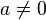
\includegraphics[scale=.6]{graphics/df44347863ac17dc898a13f44f681d01.png}.

The problem of solving a quadratic equation is a good example of how
dangerous it can be to ignore the peculiarities of floating-point
arithmetic. The obvious way to implement the quadratic formula suffers
catastrophic loss of accuracy when one of the roots to be found is much
closer to 0 than the other. In their classic textbook on numeric methods
\emph{\href{http://www.pdas.com/fmm.htm}{Computer Methods for
Mathematical Computations}}, George Forsythe, Michael Malcolm, and Cleve
Moler suggest trying the naive algorithm with \emph{a} = 1, \emph{b} = −
10\textsuperscript{5}, and \emph{c} = 1. (For double-precision floats,
set \emph{b} = − 10\textsuperscript{9}.) Consider the following
implementation in \emph{Ada}:

\begin{wideverbatim}
with Ada.Text_IO;                        use Ada.Text_IO;
with Ada.Numerics.Elementary_Functions;  use Ada.Numerics.Elementary_Functions;
 
procedure Quadratic_Equation is
   type Roots is array (1..2) of Float;
   function Solve (A, B, C : Float) return Roots is
      SD : constant Float := sqrt (B**2 - 4.0 * A * C);
      AA : constant Float := 2.0 * A;
   begin
      return ((- B + SD) / AA, (- B - SD) / AA);
   end Solve;
 
   R : constant Roots := Solve (1.0, -10.0E5, 1.0);
begin
   Put_Line ("X1 =" & Float'Image (R (1)) & " X2 =" & Float'Image (R (2)));
end Quadratic_Equation;
\end{wideverbatim}

Sample output:

\begin{verbatim}
X1 = 1.00000E+06 X2 = 0.00000E+00
\end{verbatim}

As we can see, the second root has lost all significant figures. The
right answer is that \texttt{X2} is about 10\textsuperscript{− 6}. The
naive method is numerically unstable.

Suggested by Middlebrook (D-OA), a better numerical method: to define
two parameters
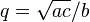
\includegraphics[scale=.6]{graphics/1b0829cacb50a2b671f2807fe80c911c.png}
and
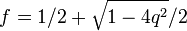
\includegraphics[scale=.6]{graphics/688bcacb300f8efe5d6d8f6411d13d96.png}

and the two roots of the quardratic are:
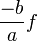
\includegraphics[scale=.6]{graphics/4bcc0c5a2bb6223fa81b5bc6f0001367.png}
and
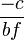
\includegraphics[scale=.6]{graphics/06242fdab96c6fc34555b2d3ac36ff56.png}

\textbf{Task}: do it better. This means that given \emph{a} = 1,
\emph{b} = − 10\textsuperscript{9}, and \emph{c} = 1, both of the roots
your program returns should be greater than 10\textsuperscript{− 11}.
Or, if your language can't do floating-point arithmetic any more
precisely than single precision, your program should be able to handle
\emph{b} = − 10\textsuperscript{6}. Either way, show what your program
gives as the roots of the quadratic in question. See page 9 of
\href{http://dlc.sun.com/pdf/800-7895/800-7895.pdf}{``What Every
Scientist Should Know About Floating-Point Arithmetic''} for a possible
algorithm.

\begin{wideverbatim}

(scl 40)

(de solveQuad (A B C)
   (let SD (sqrt (- (* B B) (* 4 A C)))
      (if (lt0 B)
         (list
            (*/ (- SD B) A 2.0)
            (*/ C 2.0 (*/ A A (- SD B) `(* 1.0 1.0))) )
         (list
            (*/ C 2.0 (*/ A A (- 0 B SD) `(* 1.0 1.0)))
            (*/ (- 0 B SD) A 2.0) ) ) ) )

(mapcar round
   (solveQuad 1.0 -1000000.0 1.0)
   (6 .) )

Output:

-> ("999,999.999999" "0.000001")

\end{wideverbatim}

\pagebreak{}
\section*{Roots of unity}

The purpose of this task is to explore working with complex numbers.
Given \texttt{n}, find the \texttt{n}-th
\href{http://en.wikipedia.org/wiki/Roots\_of\_unity}{roots of unity}.

\begin{wideverbatim}

(load "@lib/math.l")

(for N (range 2 10)
   (let Angle 0.0
      (prin N ": ")
      (for I N
         (let Ipart (sin Angle)
            (prin
               (round (cos Angle) 4)
               (if (lt0 Ipart) "-" "+")
               "j"
               (round (abs Ipart) 4)
               "  " ) )
         (inc 'Angle (*/ 2 pi N)) )
      (prinl) ) )

\end{wideverbatim}

\pagebreak{}
\section*{Rosetta Code/Count examples}


Find the total number of programming examples for each
\emph{task} and the total for all
tasks.

Essentially, count the number of occurrences of
\texttt{==\{\{header\textbar{}} on each task page.

Output:

\begin{verbatim}
100 doors: 20 examples.
99 Bottles of Beer: 29 examples.
Abstract type: 10 examples.

Total: X examples.
\end{verbatim}

\begin{wideverbatim}

(load "@lib/http.l")

(client "rosettacode.org" 80
"mw/api.php?action=query\&list=categorymembers
\&cmtitle=Category:Programming_Tasks\&cmlimit=500\&format=xml"
   (while (from " title=\"")
      (let Task (till "\"")
         (client "rosettacode.org" 80 (pack "wiki/" (replace Task " " "_"))
            (let Cnt 0
               (while (from "<span class=\"tocnumber\">")
                  (unless (sub? "." (till "<" T))
                     (inc 'Cnt) ) )
               (out NIL (prinl (ht:Pack Task) ": " Cnt)) ) ) ) ) )

Output (05may10):

100 doors: 79
24 game: 21
24 game/Solve: 15
99 Bottles of Beer: 95
A+B: 37
Abstract type: 29
...

\end{wideverbatim}

\pagebreak{}
\section*{Rosetta Code/Find unimplemented tasks}

Given the name of a language on Rosetta Code, find all tasks which are
not implemented in that language.

Note: Implementations should allow for fetching more data than can be
returned in one request to Rosetta Code.

You'll need to use the Media Wiki API, which you can find out about
locally, \href{http://rosettacode.org/mw/api.php}{here}, or in Media
Wiki's API documentation at,
\href{http://www.mediawiki.org/wiki/API\_Query}{API:Query}

\begin{wideverbatim}

(load "@lib/http.l" "@lib/xm.l")

(de rosettaCategory (Cat)
   (let (Cont NIL  Xml)
      (make
         (loop
            (client "rosettacode.org" 80
               (pack
                  "mw/api.php?action=query\&list=categorymembers\&cmtitle=Category:"
                  Cat
                  "\&cmlimit=200\&format=xml"
                  Cont )
               (while (line))
               (setq Xml (and (xml?) (xml))) )
            (NIL Xml)
            (for M (body Xml 'query 'categorymembers)
               (link (attr M 'title)) )
            (NIL (attr Xml 'query-continue' categorymembers 'cmcontinue))
            (setq Cont (pack "\&cmcontinue=" @)) ) ) ) )

(de unimplemented (Task)
   (diff
      (rosettaCategory "Programming_Tasks")
      (rosettaCategory Task) ) )

\end{wideverbatim}

\pagebreak{}
\section*{Rosetta Code/Fix code tags}

Fix Rosetta Code deprecated code tags, with these rules:

\begin{verbatim}
Change <%s> to <lang %s>
Change </%s> to </lang>
Change <code %s> to <lang %s>
Change </code> to </lang>
\end{verbatim}

Usage:

\begin{verbatim}
./convert.py < wikisource.txt > converted.txt
\end{verbatim}

\begin{wideverbatim}

#!/usr/bin/picolisp /usr/lib/picolisp/lib.l

(let Lang '("ada" "awk" "c" "forth" "prolog" "python" "z80")
   (in NIL
      (while (echo "<")
         (let S (till ">" T)
            (cond
               ((pre? "code " S) (prin "<lang" (cddddr (chop S))))
               ((member S Lang) (prin "<lang " S))
               ((= S "/code") (prin "</lang"))
               ((and (pre? "/" S) (member (pack (cdr (chop S))) Lang))
                  (prin "</lang") )
               (T (prin "<" S)) ) ) ) ) )
(bye)

\end{wideverbatim}

\pagebreak{}
\section*{Rosetta Code/Rank languages by popularity}

Sort most popular programming languages based in number of members in
Rosetta Code categories \\ (from
\href{http://www.rosettacode.org/mw/index.php?title=Special:Categories\&limit=5000}{http://www.rosettacode.org/mw/index.php?title=Special:Categories\&limit=5000})

Sample output on 6 June 2011:

\begin{verbatim}
 1.  520 - Tcl
 2.  489 - PicoLisp
 3.  479 - Python
 4.  460 - J
 5.  426 - Ruby
 6.  415 - Ada
 7.  401 - PureBasic
 8.  393 - D
 9.  385 - Haskell
10.  371 - Go
11.  366 - Java
12.  358 - OCaml
13.  357 - Perl
14.  327 - AutoHotkey
15.  322 - Common Lisp
16.  321 - C++
17.  314 - Unicon
18.  305 - Clojure
19.  289 - Icon
20.  282 - Lua
...
\end{verbatim}

Filtering wrong results is optional. You can check against
\emph{Special:MostLinkedCategories}



\begin{wideverbatim}

(load "@lib/http.l")

(for (I . X)
   (flip
      (sort
         (make
            (client "rosettacode.org" 80
               "mw/index.php?title=Special:Categories\&limit=5000"
               (while (from "<li><a href=\"/wiki/Category:")
                  (let Cat (till "\"")
                     (from "(")
                     (when (format (till " " T))
                        (link (cons @ (ht:Pack Cat))) ) ) ) ) ) ) )
   (prinl (align 3 I) ". " (car X) " - " (cdr X)) )

Output (07apr10):

  1. 390 - Tcl
  2. 389 - Programming_Tasks
  3. 359 - Python
  4. 344 - Ruby
  5. 326 - J
  6. 316 - OCaml
  7. 315 - C
  8. 312 - Haskell
  9. 296 - Perl
 10. 281 - Common_Lisp
...


Output (09aug12):

  1. 668 - Tcl
  2. 625 - PicoLisp
  3. 612 - Python
  4. 602 - C
  5. 600 - Programming_Tasks
  6. 582 - J
  7. 563 - Ruby
  8. 557 - Go
  9. 551 - Examples_needing_attention
 10. 549 - Ada
...

\end{wideverbatim}

\pagebreak{}
\section*{Rot-13}

Implement a ``rot-13'' function (or procedure, class, subroutine, or
other ``callable'' object as appropriate to your programming
environment). Optionally wrap this function in a utility program which
acts like a common \emph{UNIX} utility, performing a
line-by-line rot-13 encoding of every line of input contained in each
file listed on its command line, or (if no filenames are passed thereon)
acting as a filter on its ``standard input.'' (A number of UNIX
scripting languages and utilities, such as \emph{awk} and \emph{sed}
either default to processing files in this way or have command line
switches or modules to easily implement these wrapper semantics, e.g.,
\emph{Perl} and \emph{Python}).

The ``rot-13'' encoding is commonly known from the early days of Usenet
``Netnews'' as a way of obfuscating text to prevent casual reading of
\href{http://en.wikipedia.org/wiki/Spoiler\_(media)}{spoiler} or
potentially offensive material. Many news reader and mail user agent
programs have built-in ``rot-13'' encoder/decoders or have the ability
to feed a message through any external utility script for performing
this (or other) actions.

The definition of the rot-13 function is to simply replace every letter
of the ASCII alphabet with the letter which is ``rotated'' 13 characters
``around'' the 26 letter alphabet from its normal cardinal position
(wrapping around from ``z'' to ``a'' as necessary). Thus the letters
``abc'' become ``nop'' and so on. Technically rot-13 is a
``monoalphabetic substitution cipher'' with a trivial ``key''. A proper
implementation should work on upper and lower case letters, preserve
case, and pass all non-alphabetic characters in the input stream through
without alteration.


\begin{wideverbatim}

(de rot13-Ch (C)
   (if
      (or
         (member C '`(apply circ (chop "ABCDEFGHIJKLMNOPQRSTUVWXYZ")))
         (member C '`(apply circ (chop "abcdefghijklmnopqrstuvwxyz"))) )
      (nth @ 14 1)
      C ) )

\end{wideverbatim}

\pagebreak{}
\section*{Run as a daemon or service}

A \href{http://en.wikipedia.org/wiki/Daemon\_(computing)}{daemon} is a
service that runs in the background independent of a users login
session.

Demonstrate how a program disconnects from the terminal to run as a
daemon in the background.

Write a small program that writes a message roughly once a second to its
stdout which should be redirected to a file.

Note that in some language implementations it may not be possible to
disconnect from the terminal, and instead the process needs to be
started with stdout (and stdin) redirected to files before program
start. If that is the case then a helper program to set up this
redirection should be written in the language itself. A shell wrapper,
as would be the usual solution on Unix systems, is not appropriate.


\begin{wideverbatim}

(unless (fork)
   (out "file.log"
      (println *Pid)    # First write the daemon's PID to the file
      (for N 3600       # Write count for about one hour (if not killed)
         (wait 1000)
         (println N)
         (flush) ) )
   (bye) )              # Child terminates after one hour

(bye)                   # Parent terminates immediately

\end{wideverbatim}

\pagebreak{}
\section*{Run-length encoding}

Given a string containing uppercase characters (A-Z), compress repeated
`runs' of the same character by storing the length of that run, and
provide a function to reverse the compression. The output can be
anything, as long as you can recreate the input with it.

Example:

\begin{wideverbatim}
Input: WWWWWWWWWWWWBWWWWWWWWWWWWBBBWWWWWWWWWWWWWWWWWWWWWWWWBWWWWWWWWWWWWWW

Output: 12W1B12W3B24W1B14W
\end{wideverbatim}

Note: the encoding step in the above example is the same as a step of
the \emph{Look-and-say sequence}.


\begin{wideverbatim}

(de encode (Str)
   (pack
      (make
         (for (Lst (chop Str) Lst)
            (let (N 1  C)
               (while (= (setq C (pop 'Lst)) (car Lst))
                  (inc 'N) )
               (link N C) ) ) ) ) )

(de decode (Str)
   (pack
      (make
         (let N 0
            (for C (chop Str)
               (if (>= "9" C "0")
                  (setq N (+ (format C) (* 10 N)))
                  (do N (link C))
                  (zero N) ) ) ) ) ) )

(and
   (prinl "Data:    "
      "WWWWWWWWWWWWBWWWWWWWWWWWWBBBWWWWWWWWWWWWWWWWWWWWWWWWBWWWWWWWWWWWWWW" )
   (prinl "Encoded: " (encode @))
   (prinl "Decoded: " (decode @)) )

Output:

Data:    WWWWWWWWWWWWBWWWWWWWWWWWWBBBWWWWWWWWWWWWWWWWWWWWWWWWBWWWWWWWWWWWWWW
Encoded: 12W1B12W3B24W1B14W
Decoded: WWWWWWWWWWWWBWWWWWWWWWWWWBBBWWWWWWWWWWWWWWWWWWWWWWWWBWWWWWWWWWWWWWW

\end{wideverbatim}

\pagebreak{}
\section*{Runtime evaluation}

Demonstrate your language's ability for programs to execute code written
in the language provided at runtime. Show us what kind of program
fragments are permitted (e.g. expressions vs. statements), how you get
values in and out (e.g. environments, arguments, return values), if
applicable what lexical/static environment the program is evaluated in,
and what facilities for restricting (e.g. sandboxes, resource limits) or
customizing (e.g. debugging facilities) the execution.

You may not invoke a separate evaluator program, or invoke a compiler
and then its output, unless the interface of that program, and the
syntax and means of executing it, are considered part of your
language/library/platform.

For a more constrained task giving a specific program fragment to
evaluate, see \emph{Eval in environment}.


\begin{wideverbatim}

In PicoLisp there is a formal equivalence of code and data. Almost any peace of
data is potentially executable. PicoLisp has three internal data types: Numbers,
symbols and lists. Though in certain contexts (e.g. GUI objects) also atomic
data (numbers and symbols) are evaluated as code entities, a typical executable
item is a list.

The PicoLisp reference distinguishes between two terms: An 'exe' (expression) is
an executable list, with a function as the first element, followed by arguments.
A 'prg' (program) is a list of 'exe's, to be executed sequentially.

'exe's and 'prg's are implicit in the whole runtime system. For example, the
body of a function is a 'prg', the "true" branch of an 'if' call is an 'exe',
while the "false" branch again is a 'prg'.

For explicit execution, an 'exe' can be evaluated by passing it to the function
'[http://software-lab.de/doc/refE.html#eval eval]', while a 'prg' can be handled
by '[http://software-lab.de/doc/refR.html#run run]'.

As PicoLisp uses exclusively dynamic binding, any 'exe' or 'prg' can be executed
in arbitrary contexts. The environmet can be controlled in any conceivable way,
through implicit function parameter bindings, or explicitly with the aid of
functions like '[http://software-lab.de/doc/refB.html#bind bind]',
'[http://software-lab.de/doc/refL.html#let let]' or
'[http://software-lab.de/doc/refJ.html#job job]'.

\end{wideverbatim}

\pagebreak{}
\section*{Runtime evaluation/In an environment}

Given a program in the language (as a string or AST) with a free
variable named x (or another name if that is not valid syntax), evaluate
it with x bound to a provided value, then evaluate it again with x bound
to another provided value, then subtract the result of the first from
the second and return or print it.

Do so in a way which:

\begin{itemize}
\item
  does not involve string manipulation of the input source code
\item
  is plausibly extensible to a runtime-chosen set of bindings rather
  than just x
\item
  does not make x a \emph{global} variable
\end{itemize}

or note that these are impossible.


\begin{wideverbatim}

(let Expression '(+ X (* X X))            # Local expression
   (println
      (+
         (let X 3
            (eval Expression) )
         (let X 4
            (eval Expression) ) ) )
   (let Function (list '(X) Expression)   # Build a local function
      (println
         (+
            (Function 3)
            (Function 4) ) ) ) )

Output:

32
32

\end{wideverbatim}



% %%%%%%%%%%%%%%%%%%%%%%%% referenc.tex %%%%%%%%%%%%%%%%%%%%%%%%%%%%%%
% sample references
% %
% Use this file as a template for your own input.
%
%%%%%%%%%%%%%%%%%%%%%%%% Springer-Verlag %%%%%%%%%%%%%%%%%%%%%%%%%%
%
% BibTeX users please use
% \bibliographystyle{}
% \bibliography{}
%
\biblstarthook{In view of the parallel print and (chapter-wise) online publication of your book at \url{www.springerlink.com} it has been decided that -- as a genreral rule --  references should be sorted chapter-wise and placed at the end of the individual chapters. However, upon agreement with your contact at Springer you may list your references in a single seperate chapter at the end of your book. Deactivate the class option \texttt{sectrefs} and the \texttt{thebibliography} environment will be put out as a chapter of its own.\\\indent
References may be \textit{cited} in the text either by number (preferred) or by author/year.\footnote{Make sure that all references from the list are cited in the text. Those not cited should be moved to a separate \textit{Further Reading} section or chapter.} The reference list should ideally be \textit{sorted} in alphabetical order -- even if reference numbers are used for the their citation in the text. If there are several works by the same author, the following order should be used: 
\begin{enumerate}
\item all works by the author alone, ordered chronologically by year of publication
\item all works by the author with a coauthor, ordered alphabetically by coauthor
\item all works by the author with several coauthors, ordered chronologically by year of publication.
\end{enumerate}
The \textit{styling} of references\footnote{Always use the standard abbreviation of a journal's name according to the ISSN \textit{List of Title Word Abbreviations}, see \url{http://www.issn.org/en/node/344}} depends on the subject of your book:
\begin{itemize}
\item The \textit{two} recommended styles for references in books on \textit{mathematical, physical, statistical and computer sciences} are depicted in ~\cite{science-contrib, science-online, science-mono, science-journal, science-DOI} and ~\cite{phys-online, phys-mono, phys-journal, phys-DOI, phys-contrib}.
\item Examples of the most commonly used reference style in books on \textit{Psychology, Social Sciences} are~\cite{psysoc-mono, psysoc-online,psysoc-journal, psysoc-contrib, psysoc-DOI}.
\item Examples for references in books on \textit{Humanities, Linguistics, Philosophy} are~\cite{humlinphil-journal, humlinphil-contrib, humlinphil-mono, humlinphil-online, humlinphil-DOI}.
\item Examples of the basic Springer style used in publications on a wide range of subjects such as \textit{Computer Science, Economics, Engineering, Geosciences, Life Sciences, Medicine, Biomedicine} are ~\cite{basic-contrib, basic-online, basic-journal, basic-DOI, basic-mono}. 
\end{itemize}
}

\begin{thebibliography}{99.}%
% and use \bibitem to create references.
%
% Use the following syntax and markup for your references if 
% the subject of your book is from the field 
% "Mathematics, Physics, Statistics, Computer Science"
%
% Contribution 
\bibitem{science-contrib} Broy, M.: Software engineering --- from auxiliary to key technologies. In: Broy, M., Dener, E. (eds.) Software Pioneers, pp. 10-13. Springer, Heidelberg (2002)
%
% Online Document
\bibitem{science-online} Dod, J.: Effective substances. In: The Dictionary of Substances and Their Effects. Royal Society of Chemistry (1999) Available via DIALOG. \\
\url{http://www.rsc.org/dose/title of subordinate document. Cited 15 Jan 1999}
%
% Monograph
\bibitem{science-mono} Geddes, K.O., Czapor, S.R., Labahn, G.: Algorithms for Computer Algebra. Kluwer, Boston (1992) 
%
% Journal article
\bibitem{science-journal} Hamburger, C.: Quasimonotonicity, regularity and duality for nonlinear systems of partial differential equations. Ann. Mat. Pura. Appl. \textbf{169}, 321--354 (1995)
%
% Journal article by DOI
\bibitem{science-DOI} Slifka, M.K., Whitton, J.L.: Clinical implications of dysregulated cytokine production. J. Mol. Med. (2000) doi: 10.1007/s001090000086 
%
\bigskip

% Use the following (APS) syntax and markup for your references if 
% the subject of your book is from the field 
% "Mathematics, Physics, Statistics, Computer Science"
%
% Online Document
\bibitem{phys-online} J. Dod, in \textit{The Dictionary of Substances and Their Effects}, Royal Society of Chemistry. (Available via DIALOG, 1999), 
\url{http://www.rsc.org/dose/title of subordinate document. Cited 15 Jan 1999}
%
% Monograph
\bibitem{phys-mono} H. Ibach, H. L\"uth, \textit{Solid-State Physics}, 2nd edn. (Springer, New York, 1996), pp. 45-56 
%
% Journal article
\bibitem{phys-journal} S. Preuss, A. Demchuk Jr., M. Stuke, Appl. Phys. A \textbf{61}
%
% Journal article by DOI
\bibitem{phys-DOI} M.K. Slifka, J.L. Whitton, J. Mol. Med., doi: 10.1007/s001090000086
%
% Contribution 
\bibitem{phys-contrib} S.E. Smith, in \textit{Neuromuscular Junction}, ed. by E. Zaimis. Handbook of Experimental Pharmacology, vol 42 (Springer, Heidelberg, 1976), p. 593
%
\bigskip
%
% Use the following syntax and markup for your references if 
% the subject of your book is from the field 
% "Psychology, Social Sciences"
%
%
% Monograph
\bibitem{psysoc-mono} Calfee, R.~C., \& Valencia, R.~R. (1991). \textit{APA guide to preparing manuscripts for journal publication.} Washington, DC: American Psychological Association.
%
% Online Document
\bibitem{psysoc-online} Dod, J. (1999). Effective substances. In: The dictionary of substances and their effects. Royal Society of Chemistry. Available via DIALOG. \\
\url{http://www.rsc.org/dose/Effective substances.} Cited 15 Jan 1999.
%
% Journal article
\bibitem{psysoc-journal} Harris, M., Karper, E., Stacks, G., Hoffman, D., DeNiro, R., Cruz, P., et al. (2001). Writing labs and the Hollywood connection. \textit{J Film} Writing, 44(3), 213--245.
%
% Contribution 
\bibitem{psysoc-contrib} O'Neil, J.~M., \& Egan, J. (1992). Men's and women's gender role journeys: Metaphor for healing, transition, and transformation. In B.~R. Wainrig (Ed.), \textit{Gender issues across the life cycle} (pp. 107--123). New York: Springer.
%
% Journal article by DOI
\bibitem{psysoc-DOI}Kreger, M., Brindis, C.D., Manuel, D.M., Sassoubre, L. (2007). Lessons learned in systems change initiatives: benchmarks and indicators. \textit{American Journal of Community Psychology}, doi: 10.1007/s10464-007-9108-14.
%
%
% Use the following syntax and markup for your references if 
% the subject of your book is from the field 
% "Humanities, Linguistics, Philosophy"
%
\bigskip
%
% Journal article
\bibitem{humlinphil-journal} Alber John, Daniel C. O'Connell, and Sabine Kowal. 2002. Personal perspective in TV interviews. \textit{Pragmatics} 12:257--271
%
% Contribution 
\bibitem{humlinphil-contrib} Cameron, Deborah. 1997. Theoretical debates in feminist linguistics: Questions of sex and gender. In \textit{Gender and discourse}, ed. Ruth Wodak, 99--119. London: Sage Publications.
%
% Monograph
\bibitem{humlinphil-mono} Cameron, Deborah. 1985. \textit{Feminism and linguistic theory.} New York: St. Martin's Press.
%
% Online Document
\bibitem{humlinphil-online} Dod, Jake. 1999. Effective substances. In: The dictionary of substances and their effects. Royal Society of Chemistry. Available via DIALOG. \\
http://www.rsc.org/dose/title of subordinate document. Cited 15 Jan 1999
%
% Journal article by DOI
\bibitem{humlinphil-DOI} Suleiman, Camelia, Daniel C. O�Connell, and Sabine Kowal. 2002. `If you and I, if we, in this later day, lose that sacred fire...�': Perspective in political interviews. \textit{Journal of Psycholinguistic Research}. doi: 10.1023/A:1015592129296.
%
%
%
\bigskip
%
%
% Use the following syntax and markup for your references if 
% the subject of your book is from the field 
% "Computer Science, Economics, Engineering, Geosciences, Life Sciences"
%
%
% Contribution 
\bibitem{basic-contrib} Brown B, Aaron M (2001) The politics of nature. In: Smith J (ed) The rise of modern genomics, 3rd edn. Wiley, New York 
%
% Online Document
\bibitem{basic-online} Dod J (1999) Effective Substances. In: The dictionary of substances and their effects. Royal Society of Chemistry. Available via DIALOG. \\
\url{http://www.rsc.org/dose/title of subordinate document. Cited 15 Jan 1999}
%
% Journal article by DOI
\bibitem{basic-DOI} Slifka MK, Whitton JL (2000) Clinical implications of dysregulated cytokine production. J Mol Med, doi: 10.1007/s001090000086
%
% Journal article
\bibitem{basic-journal} Smith J, Jones M Jr, Houghton L et al (1999) Future of health insurance. N Engl J Med 965:325--329
%
% Monograph
\bibitem{basic-mono} South J, Blass B (2001) The future of modern genomics. Blackwell, London 
%
\end{thebibliography}

